\section{Algoritmo Exacto}
De acuerdo a lo ya explicado en el inciso \ref{caballitos}, podemos establecer una analog\'ia con este problema y ``El se\~nor de los caballos''. Por lo tanto, la metodolog\'ia empleada para la implementaci\'on del algoritmo exacto tambi\'en fue la de \emph{Backtracking}.\\

De este modo, nos vemos obligados a recorrer inteligentemente todos los conjuntos dentro del conjunto de partes del total de nodos $V$. Mediante el backtracking podemos realizar podas y estrategias para saltear algunas ramas de decisi\'on donde se predice que no se va a poder encontrar la soluci\'on \'optima all\'i.


\subsection{Explicaci\'on y mejoras}
%Explicar detalladamente el algoritmo implementado. Elaborar podas y estrategias que permitan mejorar los tiempos de resolucion.

Nuestro algoritmo recorre ordenadamente el conjunto de partes de V y por cada uno de ellos verifica que cumpla la funci\'on  \texttt{esIndependienteMaximal()}. La misma devuelve 0 si es falso, la cantidad de nodos en el conjunto en caso contrario.\\

Es decir, se itera sobre los nodos y, considerando el nodo actual como presente o como ausente, termina encontrando el m\'inimo conjunto independiente maximal.\\

En una variable se acumula la soluci\'on \'optima hasta el momento, la cual se actualiza cuando se encuentra un nuevo conjunto independiente maximal que tiene un cardinal menor al \'optimo actual. 
En ella va a quedar la soluci\'on buscada luego de correr el algoritmo.\\

La poda que implementamos consisti\'o en verificar que una futura soluci\'on posible no cuente con una cantidad igual o superior de nodos que la soluci\'on \'optima obtenida hasta el momento. 
Esto quiere decir que si la \'optima actual consiste de $k$ nodos y nos encontramos ante la pregunta de agregar un nuevo nodo a una posible soluci\'on de $k - 1$ nodos, \'esta ser\'a a lo sumo 
tan buena como la que ya ten\'iamos, por lo que no nos resulta \'util contemplarla. De esta forma, se descartan r\'apidamente todas las soluciones peores o iguales que la actual.\\

Otra poda posible consist\'ia en separar cada una de las componentes conexas del grafo y, para cada una de ellas, buscar el m\'inimo conjunto independiente maximal.
Luego, uniendo todos estos resultados, se obtiene el conjunto deseado del grafo.\\

Una estrategia podr\'ia ser verificar si agregar el nodo actual me va a resultar \'util. Es decir, por ejemplo, si estoy agregando un vecino de un nodo que ya se encuentra en el conjunto, este no ser\'a \'util ya que
la soluci\'on no ser\'ia maximal. De esta forma, podr\'iamos evitar revisar aquellos conjuntos.\\

Estas dos optimizaciones no se implementaron porque requer\'ian un manejo distinto de estructuras lo cual consideramos ser\'ia innecesario ya que empeorar\'ian los tiempos de ejecuci\'on.

\newpage
\begin{algorithm}[h!]
\caption{algoritmo exacto}

\textit{unsigned int} \textbf{calcularCIDM}(Matriz\& \textit{adyacencia}, unsigned int \textit{i}, vector$<$unsigned int$>$\& \textit{conjNodos}, vector$<$unsigned int$>$\& \textit{optimo})\{ 
\newline

\If{(conjNodos.esIndependienteMaximal())}{
		optimo $\longleftarrow$ conjNodos;\\
		\textbf{return} optimo.size();
}
\If{(i.estaEnRango())}{
	\If{(conjNodos es m\'as grande que el optimo actual)}{
		\textbf{return} 0;
	}
	siNoAgrego $\longleftarrow$ calcularCIDM(adyacencia, i+1, conjNodos, optimo);\\
	agrego el nodo $i$ a conjNodos;\\
	siAgrego $\longleftarrow$ calcularCIDM(adyacencia, i+1, conjNodos, optimo);\\
	elimino el nodo $i$ de conjNodos;\\
	\textbf{return} el mejor entre $siNoAgrego$ y $siAgrego$;
}
\textbf{return} 0;
\end{algorithm}

\subsection{Complejidad Temporal}
%Calcular el orden de complejidad temporal de peor caso del algoritmo.
Al ser un algoritmo de $Backtracking$ o fuerza bruta, tiene una complejidad exponencial. En este caso, la misma es de $O(2^n)$, siendo $n$ la cantidad de nodos del grafo. \\

Se llega a dicha complejidad dado que para cada nodo, tenemos que preguntarnos qu\'e ocurre tanto si lo agregamos al conjunto, como si no.\\

Dicho de otra forma, vamos a recorrer todos los conjuntos dentro del conjunto de partes del total de nodos de $V$. El cardinal de dicho conjunto de partes es $2^n$.\\

Para cada uno de los subconjuntos, el algoritmo verifica si cumple la funci\'on \texttt{esIndependienteMaximal()}, la cual
tiene una complejidad en peor caso de $O(n^2)$.	De esta forma, nuestro algoritmo tiene complejidad $O(2^n * n^2)$, lo que es equivalente a $O(2^n)$.\\

Al tener en cuenta la poda utilizada, se puede ver que la misma no disminuye la complejidad te\'orica planteada dado que en el peor caso, podr\'ia haber que recorrer completamente el conjunto de partes.
De todas formas, dicha poda mejora notablemente los tiempos de ejecuci\'on del algoritmo, como veremos m\'as adelante, ya que descarta las soluciones peores que la \'optima hasta el momento.\\

\newpage
\subsection{Experimentaci\'on}
%Realizar una experimentacion que permita observar los tiempos de ejecucion del algoritmo en funcion de los parametros de la entrada y de las podas y/o estrategias implementadas.
Para realizar la experimentaci\'on, se genereron grafos espec\'ificos, que nos permitieron ver el funcionamiento de nuestro algoritmo.
Las conexiones entre los nodos de cada grafo son aleatorias, pero respetando la cantidad de ejes que nosotros definamos previamente.\\

Las instancias con tiempos de ejecuci\'on bajos fueron corridas 100 veces, obteni\'endo luego un promedio de todas, con el fin de eliminar outliers.
Aquellas instancias que tardaban mucho m\'as tiempo, determinamos que los outliers no modificaban en forma considerable, por lo que no nos pareci\'o necesario realizarlas reiteradas veces.

\subsubsection{Mejor caso}
De acuerdo a c\'omo fue planteado nuestro algoritmo, se puede ver que el mejor caso posible ser\'a cuando los grafos pasados por par\'ametro sean completos.
Esto es as\'i debido a la poda implementada: cuando considera al primer nodo, encuentra una posible soluci\'on y luego descarta r\'apidamente todas las dem\'as, ya que una soluci\'on con un solo nodo 
ser\'a necesariamente una soluci\'on \'optima.\\

  \begin{figure}[h!]
   \begin{center}
 	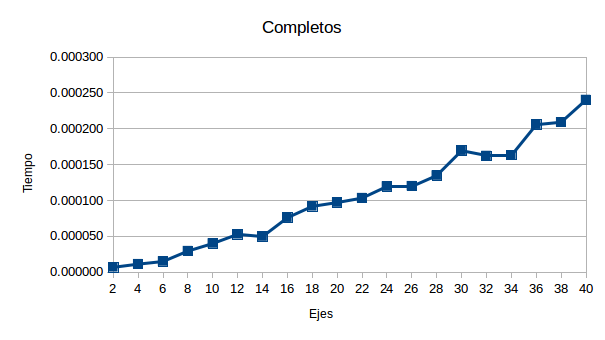
\includegraphics[scale=0.7]{imagenes/exacto/Completos.png}
% 	\caption{}
%	\label{GrafoCompleto}
   \end{center}
 \end{figure}

Se puede ver que el gr\'afico no tiene una tendencia exponencial, lo que era esperable ya que encontrar\'a la soluci\'on en el primer nodo, pero luego deber\'a descartar los siguientes $n$ nodos,
teniendo una complejidad en peor caso de $O(n^2)$.\\

\newpage

\subsubsection{Nodos fijos}
Para continuar viendo el comportamiento del algoritmo, decidimos realizar experimentos fijando la cantidad de nodos y variando la cantidad de ejes.\\

Los tiempos de ejecuci\'on para nodos fijos en 10 fueron los siguientes:\\

  \begin{figure}[h!]
   \begin{center}
\begin{tabular}{| l | l |}
  \hline
  Ejes & Tiempo \\ \hline
  0 & 0.00183446 \\ \hline
  5 & 0.00144151 \\ \hline
  10 & 0.00109473 \\ \hline
  15 & 0.00016757 \\ \hline
  20 & 0.00026461 \\ \hline
  25 & 0.00002951 \\ \hline
  30 & 0.00002110 \\ \hline
  35 & 0.00002912 \\ \hline
  40 & 0.00003069 \\ \hline
  45 & 0.00002226 \\ \hline
\end{tabular}
   \end{center}
 \end{figure}
 
  \begin{figure}[h!]
   \begin{center}
 	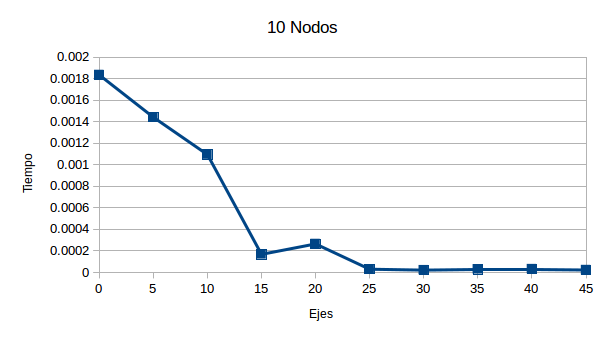
\includegraphics[scale=0.7]{imagenes/exacto/10Nodos.png}
% 	\caption{}
%	\label{10Nodos}
   \end{center}
 \end{figure}

\newpage
 Tiempos para 20 nodos: \\

  \begin{figure}[h!]
   \begin{center}
 \begin{tabular}{| l | l |}
 \hline
  Ejes & Tiempo \\ \hline
  0 & 2.711875 \\ \hline
  10 & 2.0401455 \\ \hline
  20 & 1.3764805 \\ \hline
  30 & 0.076818295 \\ \hline
  40 & 0.05422746 \\ \hline
  50 & 0.009414217 \\ \hline
  60 & 0.025866655 \\ \hline
  70 & 0.0009003714 \\ \hline
  80 & 0.0049536455 \\ \hline
  90 & 0.0019486415 \\ \hline
  100 & 0.0037668155 \\ \hline
  110 & 0.000811313 \\ \hline
  120 & 0.001422941 \\ \hline
  130 & 0.0001214862 \\ \hline
  140 & 0.0001463258 \\ \hline
  150 & 9.03317E-005 \\ \hline
  160 & 0.0001304291 \\ \hline
  170 & 0.0001313739 \\ \hline
  180 & 0.000095395 \\ \hline
 \end{tabular}
   \end{center}
 \end{figure}

  \begin{figure}[h!]
   \begin{center}
 	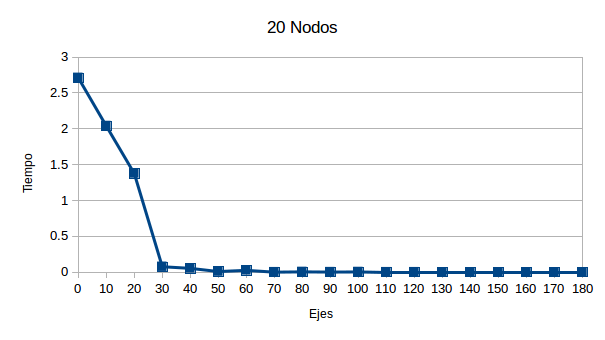
\includegraphics[scale=0.7]{imagenes/exacto/20Nodos.png}
% 	\caption{}
%	\label{20Nodos}
   \end{center}
 \end{figure}
 
 \newpage
 Para 30 nodos: \\
   \begin{figure}[h!]
   \begin{center}
\begin{tabular}{| l | l |}
  \hline
  Ejes & Tiempo \\ \hline
  0 & 3854.93 \\ \hline
  5 & 3004.21 \\ \hline
  10 & 3035.02 \\ \hline
  15 & 2276.72 \\ \hline
  20 & 2423.98 \\ \hline
  25 & 2026.34 \\ \hline
  30 & 645.834 \\ \hline
  35 & 173.097 \\ \hline
  40 & 199.783 \\ \hline
  45 & 93.6673 \\ \hline
  50 & 285.263 \\ \hline
  55 & 37.6866 \\ \hline
  60 & 46.629645 \\ \hline
  65 & 33.144255 \\ \hline
  70 & 11.19414 \\ \hline
  75 & 15.869275 \\ \hline
  80 & 7.440072 \\ \hline
  85 & 1.420106 \\ \hline
  90 & 3.3511875 \\ \hline
  95 & 1.2927065 \\ \hline
  100 & 1.0168595 \\ \hline
  105 & 0.15861015 \\ \hline
  110 & 0.4207426 \\ \hline
\end{tabular}
   \end{center}
 \end{figure}

   \begin{figure}[h!]
   \begin{center}
 	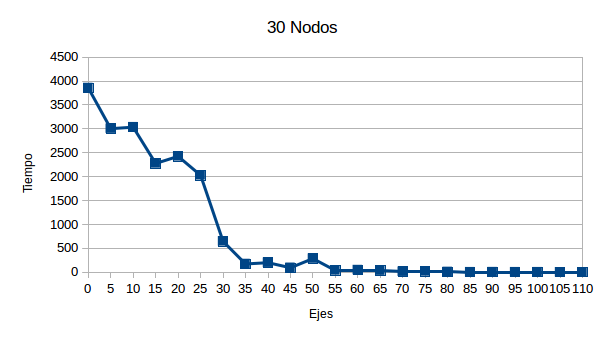
\includegraphics[scale=0.7]{imagenes/exacto/30Nodos.png}
% 	\caption{}
%	\label{30Nodos}
   \end{center}
 \end{figure}
 
Como podemos ver, en todos los casos ocurre algo similar: cuando no tienen ejes la ejecuci\'on es m\'as lenta, ya que debe recorrer todas las posibles opciones del conjunto de partes, sin lograr descartar ninguna.
A medida que se van agregando ejes, los tiempos van decreciendo ya que gracias a la poda implementada, no es necesario recorrer todas las posibles soluciones.\\

\subsubsection{Ejes fijos}
En esta secci\'on podremos ver el comportamiento exponencial del ejercicio, ya que se mantuvo fija la cantidad de ejes, pero fue aumentando la cantidad de nodos.
Los resultados de los tiempos de ejecucion, con 45 ejes fijos fueron:\\
 \begin{figure}[h!]
   \begin{center}
\begin{tabular}{| l | l |}
\hline
 Nodos & Tiempo  \\ \hline
10 & 6.974115E-005 \\ \hline
12 & 0.0001912309 \\ \hline
14 & 0.0001047463 \\ \hline
16 & 0.010293569 \\ \hline
18 & 0.013017305 \\ \hline
20 & 0.023726705 \\ \hline
22 & 0.13164895 \\ \hline
24 & 0.4864227 \\ \hline
26 & 20.211575 \\ \hline
28 & 44.99018 \\ \hline
30 & 344.1135 \\ \hline
32 & 3090.602 \\ \hline
34 & 2977.318 \\ \hline
36 & 7641.97 \\ \hline
38 & 49532.4333333333 \\ \hline
\end{tabular}
   \end{center}
 \end{figure}


 \begin{figure}[h!]
   \begin{center}
 	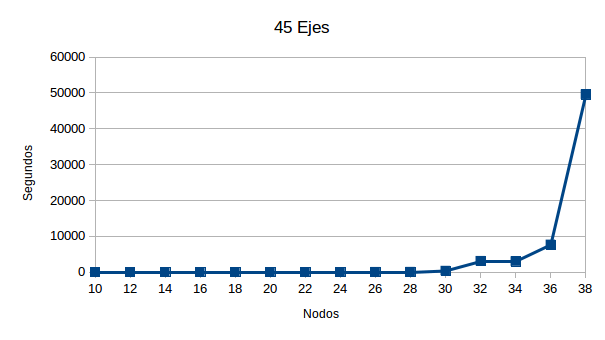
\includegraphics[scale=0.7]{imagenes/exacto/45Ejes.png}
% 	\caption{}
%	\label{45Ejes}
   \end{center}
 \end{figure}
 
\newpage 
 Para 90 ejes: \\
 
 \begin{figure}[h!]
   \begin{center}
 \begin{tabular}{| l | l |}
  \hline
Nodos & Tiempo \\ \hline
15 & 6.50116E-005 \\ \hline
17 & 0.0004393166 \\ \hline
19 & 0.0006342648 \\ \hline
21 & 0.033956355 \\ \hline
23 & 0.02623205 \\ \hline
25 & 0.042124215 \\ \hline
27 & 0.11144235 \\ \hline
29 & 0.75794095 \\ \hline
31 & 9.9156506667 \\ \hline
33 & 24.44762 \\ \hline
 \end{tabular}
   \end{center}
 \end{figure}
 
 
 \begin{figure}[h!]
   \begin{center}
 	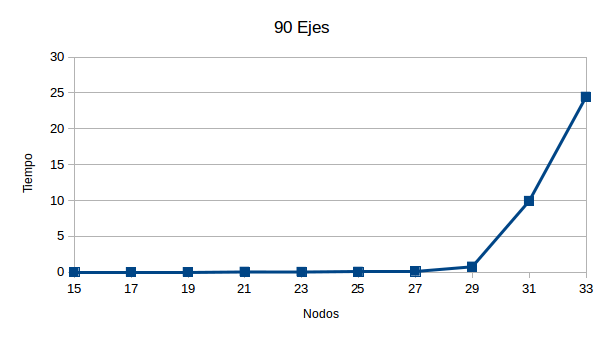
\includegraphics[scale=0.7]{imagenes/exacto/90Ejes.png}
% 	\caption{}
%	\label{30Nodos}
   \end{center}
 \end{figure}
 
Como preve\'iamos, se puede ver que los valores van aumentando exponencialmente en ambos casos, lo cual nos indica que la complejidad temporal depende directamente de la cantidad de nodos que tenga
el grafo.
De todas formas, en algunos casos es posible ver el efecto que tiene la poda, ya que el tiempo de ejecuci\'on no aument\'o exponencialmente, por ejemplo, entre los casos con 32 y 34 nodos, con 45 ejes fijos.
Veremos luego que esto no ocurre en el peor caso.\\

Para mostrar m\'as claramente el aspecto exponencial de la funci\'on en los casos m\'as chicos, haremos zoom en el gr\'afico:\\

\begin{figure}[h!]
   \begin{center}
 	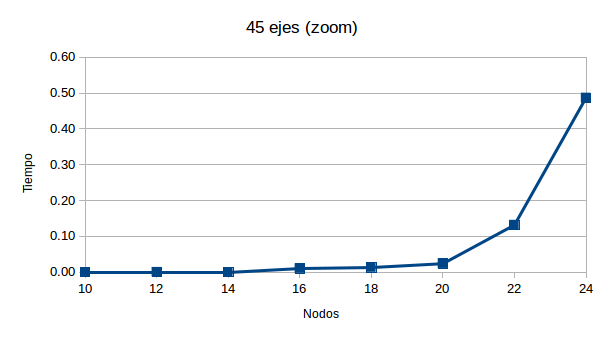
\includegraphics[scale=0.7]{imagenes/exacto/45Ejes(zoom).png}
% 	\caption{}
%	\label{45Ejes}
   \end{center}
 \end{figure}

\subsubsection{Sin ejes}
El peor caso para nuestro algoritmo se da cuando el grafo pasado por par\'ametro no cuenta con ning\'un eje. Esto es as\'i porque deber\'a revisar todos los posibles conjuntos dentro del conjunto de partes,
intentando encontrar uno mejor que el que utiliza todos los nodos. Claramente esto no es posible, ya que al no contar con ejes, aquella es la \'unica soluci\'on posible.\\

\newpage
Los tiempos de ejecuci\'on para los distintos grafos sin ejes fueron:\\

   \begin{figure}[h!]
   \begin{center}
 	\begin{tabular}{| l | l |}
 \hline
Nodos & Tiempo \\ \hline
2 & 5.4496E-006 \\ \hline
4 & 3.91842E-005 \\ \hline
6 & 0.0002040706 \\ \hline
8 & 0.0006613658 \\ \hline
10 &  0.002856698 \\ \hline
12 &  0.00857044 \\ \hline
14 &  0.03590956 \\ \hline
16 &  0.1578688 \\ \hline
18 &  0.681332 \\ \hline
20 &  2.930954 \\ \hline
22 &  12.58866 \\ \hline
24 &  53.82 \\ \hline
26 &  229.522 \\ \hline
\end{tabular}
\end{center}
 \end{figure}
 

   \begin{figure}[h!]
   \begin{center}
 	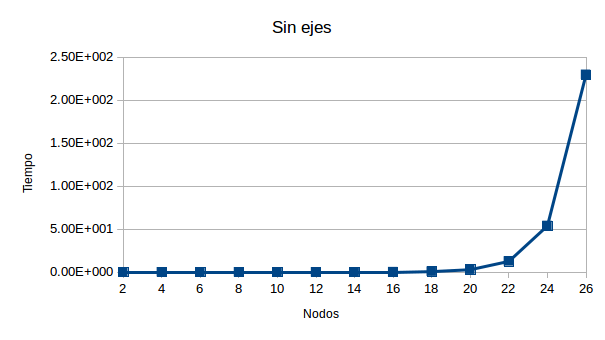
\includegraphics[scale=0.7]{imagenes/exacto/Vacios.png}
% 	\caption{}
%	\label{Vacio}
   \end{center}
 \end{figure}
 
\newpage 
 
Para ver m\'as claramente el aspecto del gr\'afico para los casos m\'as chicos, haremos zoom en el gr\'afico:\\

\begin{figure}[h!]
   \begin{center}
 	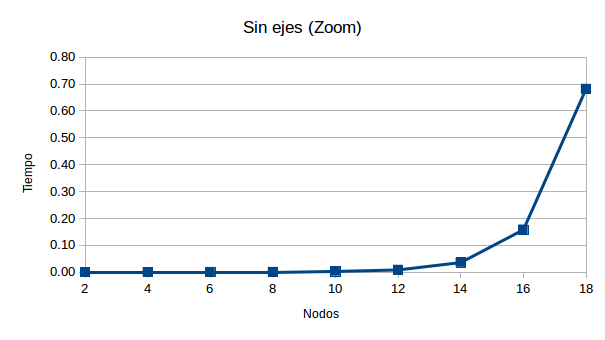
\includegraphics[scale=0.7]{imagenes/exacto/Vacio(zoom).png}
% 	\caption{}
%	\label{45Ejes}
   \end{center}
 \end{figure}

Aqu\'i se ve claramente que los tiempos aumentan exponencialmente en cada paso, lo que confirma nuestra complejidad temporal te\'orica de $O(2^n)$.\\
